\chapter{Background}
\label{chp:background}

\section{Internet of Things}

What is iot.

Device-to-device communication

Where is it going

Security challenges


\section{The IEEE 802.15.4 Standard}

Following the evolution of \gls{iot}, the need for cheap devices to communicate efficiently between each other has arose. Existing architectures such as 802.11 (WiFi) and Bluetooth are too expensive in terms of processing and energy consumption, as the idea of \gls{iot} is to connect even the smallest devices to a network or Internet. As these devices are small, they have a limited amount of battery, and hence need to use it in a highly efficient matter.

\begin{wrapfigure}[12]{r}{0pt}
  \centering
  \includegraphics[scale=0.55]{osi} %Note: no use of .jpg file ending
  \vspace{-0.2cm}
  \caption{The \gls{osi} stack with layers, the data they carry, and some of the most known technologies for the different layers. Note that layer 5 (Session), 6 (Presentation) and 7 (Application) have been merged into one layer.}
  \label{fig:osi}
\end{wrapfigure}
802.15.4 protocols are envisioned for applications supporting smart homes, medical surveillance, monitoring systems for environmental and industrial systems, as well as sensor systems for heating and ventilation. As we know from the \gls{iot}, it is really the imagination that puts and end to the possibilities for interconnected devices. The \gls{osi} stack defines the internal structure of communications systems, and is shown in Figure \ref{fig:osi}. In this figure, layer 5, 6 and 7 are merged into the same layer for simplicity.

As the 802.15.4 standard only defines the physical and data link (\gls{mac}) layer of the \gls{osi} stack, specifications need to be developed to utilize the possibilities provided by 802.15.4 in the upper layers. ZigBee, maintained by the ZigBee Alliance, is the most notable example of specifications that uses 802.15.4 as its base. Others include WirelessHART, MiWi, and ISA100.11a. Cite these? Homepage?
% cite

The fundamental intention of the 802.15.4 standard is to provide low-rate, low-power communication between devices within a sensor network or \gls{wpan}. Its main use case is to let multiple devices within a short range communicate with each other over a low-rate radio, while maintaining a modest energy consumption. Figure \ref{fig:802154-figure} paints a picture of what 802.15.4 is compared to more well-established concepts such as WiFi (802.11) and Bluetooth. While being a smaller, more cost efficient device than those found in more complex networks, 802.15.4 networks have a much more limited range (about 10 meters), and in most cases a throughput below 250 Kbps \cite{gutierrez2001ieee}. Not only is the 802.15.4 standard significantly lighter in terms of data rate and power consumption, it is also aimed on a different market than regular \gls{wpan}s. \gls{wpan}s are oriented around a person, creating a personal network for the user, which has higher demands to data rate, and can allow a higher energy consumption. 802.15.4, however, focuses on interconnecting devices that do not necessary have this constraint, such as industrial and medical applications. 


\begin{figure}
	\centering
	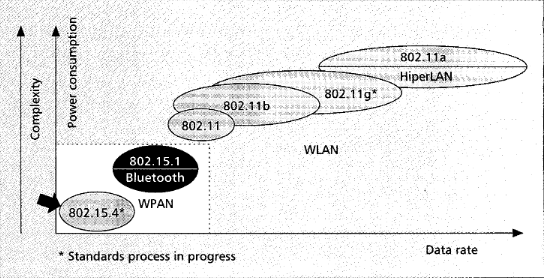
\includegraphics[scale=0.85]{802-15-4-place.png}
	\caption{Figure of IEEE 802.15.4's operational space compared to other wireless standards \cite{gutierrez2001ieee}.}
	\label{fig:802154-figure}
\end{figure}


From a security point of view, the 802.15.4 standard provides two of the properties in the \gls{cia} triad, namely confidentiality and integrity, through its link-layer security package \cite{sastry2004security}. When seen in conjunction with possible use cases for 802.15.4, these are important features. For sensor networks related to medical facilities, data confidentiality protects sensitive information about patients from being disclosed to unauthorized parties. Data integrity protects the data from being tampered with, which can cause serious harm for all sorts of sensor networks and applications.


Four basic security services are provided in the 802.15.4 link-layer security package, namely access control, message integrity, message confidentiality and replay protection (sequential freshness). 802.15.4 is delivered with a total of eight different security suites, providing none, some or all of the described security services. In the most secure end of the scale we find \gls{aes}-\gls{ccm}, which is encryption with either 32, 64 or 128-bit \gls{mac-auth}. 

 


Access control and replay protection filters out packages at the link layer.

Git


\section{6LoWPAN: Putting IP on Top of 802.15.4}

% We want to reach our devices over the Internet. IP is the thing.


Initially, the \gls{ip} was considered to be too "heavy" for low-power wireless networks such as the ones described by the 802.15.4 standard. The idea of implementing \gls{ip} on top of 802.15.4 networks was born as early as in 2001 under the question "Why invent a new protocol when we already have IP?"\cite{Mulligan2007}. With \gls{ip}, the community already had a bundle of existing protocols for management, transport, configuring and debugging, such as \gls{snmp}, \gls{tcp} and \gls{udp}, as well as standardized services for higher layers such as caching, firewalls, load balancing and mobility. Nevertheless, the initial idea of using IP in combination with sensor networks or \gls{wpan} was not accepted by various groups such as ZigBee \cite{Mulligan2007}. The rejection did, however, not stop the initiative, and a group of engineers within \gls{ietf} started designing and developing what would later be known as \gls{6lowpan}.

Another significant advantage with combining \gls{ip} and 802.15.4 is the simplification of the connectivity model between various devices in the networks. As most 802.15.4-based specifications usually needs custom hardware that tend to be complex, the possibilities to interconnect different networks with each other is somewhat limited. By turning to \gls{ip}, the need for complex connectivity models is obviate as it is possible to use well-understood technologies such as bridges and routers. Another advantage with using \gls{ip} is that the routers between the \gls{6lowpan} devices and the outside networks (so-called edge routers) do not need to maintain any state as they are only forwarding datagrams.

The implementation of \gls{6lowpan} proved to not be any more expensive compared to other alternatives such as ZigBee or Z-wave in terms of code size and \gls{ram} requirements \cite{Mulligan2007}. Another important feature of \gls{6lowpan}

New features - Why is this doable over IP?

Encapsulation and header compression. 

Supports common topologies such as star and mesh.

\gls{6lowpan} uses, as stated in its acronym, IPv6.

Unique concept: Only pay for what you use in terms of overhead and processing because of a new header compressing mechanism.


% WHY ARE WE TALKING ABOUT THIS?

Security considerations.


% Security part

\section{Formal Security Analysis} 


As security protocols grows larger and more complex, they become more and more difficult for humans to analyse. One of the examples of the need for formal security analysis, is the Needham-Schroeder protocol \cite{Needham:1978} from 1978. The Needham-Schroeder protocol is based on public-key cryptography and was intended to allow two communicating parties to mutual authenticate each other.

Initially, the security protocol analysis was conducted using so-called \gls{ban} logic, which showed promising results in finding security flaws and drawbacks for several authentication protocols, along with proving that the Needham-Schroeder protcol was, in fact, secure \cite{burrows1989logic}. \gls{ban} logic is a set of rules which can be used to determine whether received information is legit or not by formally describe the interaction between communicating parties. 

17 years later, after being deployed and widely used, G. Lowe discovered, using the automatic tool Casper, that the Needham-Schroeder protocol was in fact insecure, and vulnerable to a man-in-the-middle attack \cite{lowe1996}. Formal security analysis gained increased interest from the research community after the discovery by Lowe, and ... More....

The Dolev-Yao model is a formal model used to prove the security properties of cryptographic protocols. While initially being a verification model built for public key protocols, the Dolev-Yao model is also the basis for most of the security analysis done by verification tools \cite{cremers2005operational}. The model is built upon three primary assumptions \cite{dolev1983security}. Firstly, the Dolev-Yao model assumes that the cryptography is perfect, essentially meaning that the cryptographic system can not be tampered with, and an encrypted message can only be decrypted by the party possessing the corresponding decryption key. The second assumption is that the adversary has completely control over the communication network, hence he is able to observe all messages that are sent between communicating parties, and can inject messages given that he is able to forge its content in a valid matter. Lastly, messages that are sent in the network are to be observed as abstract terms, where the attacker has two possible outcomes; either he learns the complete content of the message, or he learns nothing at all. 

More to come.


